\documentclass{standalone}
\usepackage{tikz}
\begin{document}
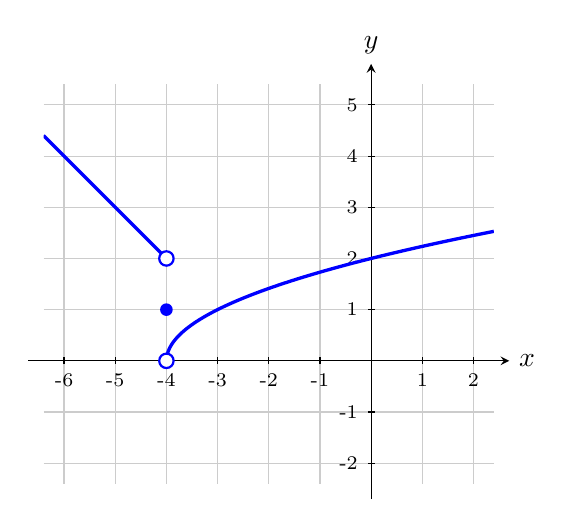
\begin{tikzpicture}[>=stealth, scale=0.65]
  % Grid
  \draw[gray!40, thin] (-6.4,-2.4) grid (2.4,5.4);
  % Axes
  \draw[->] (-6.7,0) -- (2.7,0) node[right] {$x$};
  \draw[->] (0,-2.7) -- (0,5.8) node[above] {$y$};
  % x-axis ticks and labels
  \foreach \x in {-6,-5,-4,-3,-2,-1,1,2} {
    \draw (\x,0.07) -- (\x,-0.07) node[below, font=\scriptsize] {\x};
  }
  % y-axis ticks and labels
  \foreach \y in {-2,-1,1,2,3,4,5} {
    \draw (0.07,\y) -- (-0.07,\y) node[left, font=\scriptsize] {\y};
  }
  % Piecewise function:
  %   left branch:  y = -(x + 4) + 2 = -x - 2   (x < -4), open circle at (-4,2)
  %   defined value: f(-4) = 1, filled dot at (-4,1)
  %   right branch: y = sqrt(x + 4)             (x > -4), open circle at (-4,0)
  \begin{scope}
    \clip (-6.4,-2.4) rectangle (2.4,5.4);
    \draw[blue, very thick, domain=-6.4:-4] plot (\x, {-\x - 2});
    \draw[blue, very thick, samples=200, domain=-4:2.4] plot (\x, {sqrt(\x + 4)});
  \end{scope}
  % Open circles (limit values)
  \draw[fill=white, draw=blue, thick] (-4,2) circle (4pt);
  \draw[fill=white, draw=blue, thick] (-4,0) circle (4pt);
  % Filled dot (defined value)
  \fill[blue] (-4,1) circle (3.5pt);
\end{tikzpicture}
\end{document}
